\chapter{The Proposed 3D Head Motion Tracking}
\label{c:method}

% ------------------------ %
%                          %
% Rigid Body Motion Module %
%                          %
% ------------------------ %
\section{Rigid Body Motion Module}
In our work, we assume the subject human head is a rigid body where none of its points have relative motions respect to one another. In other words, every point on the rigid body must always maintain a fixed position relative to one another. All the points move with each other together as a whole. Therefore, the motion of every point on the rigid body can be represented by the same translation and rotation transformation. Then we can infer that there exist a rotation matrix $R$ and a translation matrix $T$ such that for all points $p$ on the rigid body and its corresponding position $p'$ after the transformation satisfy the following equation:
\begin{equation}
p' = Rp + T
\label{e:rbt}
\end{equation}
or
\begin{equation}
\begin{bmatrix}
x'\\y'\\z'
\end{bmatrix}
=
\begin{bmatrix}
r_{11}&r_{12}&r_{13}\\
r_{21}&r_{22}&r_{23}\\
r_{31}&r_{32}&r_{33}
\end{bmatrix}
\begin{bmatrix}
x\\y\\z
\end{bmatrix}
+
\begin{bmatrix}
t_{x}\\t_{y}\\t_{z}
\end{bmatrix}
\end{equation}
Borrowing aviation terminology, the rotation terms are commonly referred to as pitch, yaw, and roll. A pitch is a counter-clockwise rotation of $\theta$ around the $x$-axis. The rotation matrix is given by:
\begin{equation}
R(x)=
\begin{bmatrix}
1&0&0\\
0&\cos\theta & -\sin\theta \\
0&\sin\theta & \cos\theta
\end{bmatrix}
\end{equation}
A yaw is a counter-clockwise rotation of $\psi$ around the $y$-axis. The rotation matrix is given by:
\begin{equation}
R(y)=
\begin{bmatrix}
\cos\psi & 0 & \sin\psi \\
0&1&0\\
-\sin\psi &0 & \cos\psi
\end{bmatrix}
\end{equation}
A roll is a counter-clockwise rotation of $\phi$ around the $z$-axis. The rotation matrix is given by:
\begin{equation}
R(z)=
\begin{bmatrix}
\cos\phi & -\sin\phi & 0\\
\sin\phi & \cos\phi & 0\\
1&0&0
\end{bmatrix}
\end{equation}
The pitch, yaw, and roll rotations can be used to represent any orientation of the rigid body. The single rotation matrix in Equation \ref{e:rbt} can be formed by multiplying the above three matrices, then we obtain:
\begin{equation}
R=R(\theta)R(\psi)R(\phi)=
\begin{bmatrix}
1&0&0\\
0&\cos\theta & -\sin\theta \\
0&\sin\theta & \cos\theta
\end{bmatrix}
\begin{bmatrix}
\cos\psi & 0 & \sin\psi \\
0&1&0\\
-\sin\psi &0 & \cos\psi
\end{bmatrix}
\begin{bmatrix}
\cos\phi & -\sin\phi & 0\\
\sin\phi & \cos\phi & 0\\
1&0&0
\end{bmatrix}
\end{equation}

% ------------------------ %
%                          %
% Point Clouds Generation  %
%                          %
% ------------------------ %
\section{Point Clouds Generation}
\label{s:point cloud gen}
The proposed system adopts Microsoft Kinect to caputre the deoth information. A depth map in VGA resolution is generated with pixel values ranging from 0 to 10000 millimeters. Our task is to obtain the corresponding 3D vertex $p_{3D}(x,y,z)$ of each pixel $P_{2D}(X,Y)$ on the depth map (Figure \ref{f:pcGenerate}). Regarding the depth value of each pixel to be its z-coordinate, we still need to calculate the x- and y-coordinates.
\begin{figure}
\centering
\includegraphics[width=1.0\linewidth]{./figure/pcGenerate.pdf}
\caption{Flow chart of procedure \emph{point cloud generation}. The input is a depth map and the output is the corresponding 3D point set.}
\label{f:pcGenerate}
\end{figure}
\begin{figure}
\centering
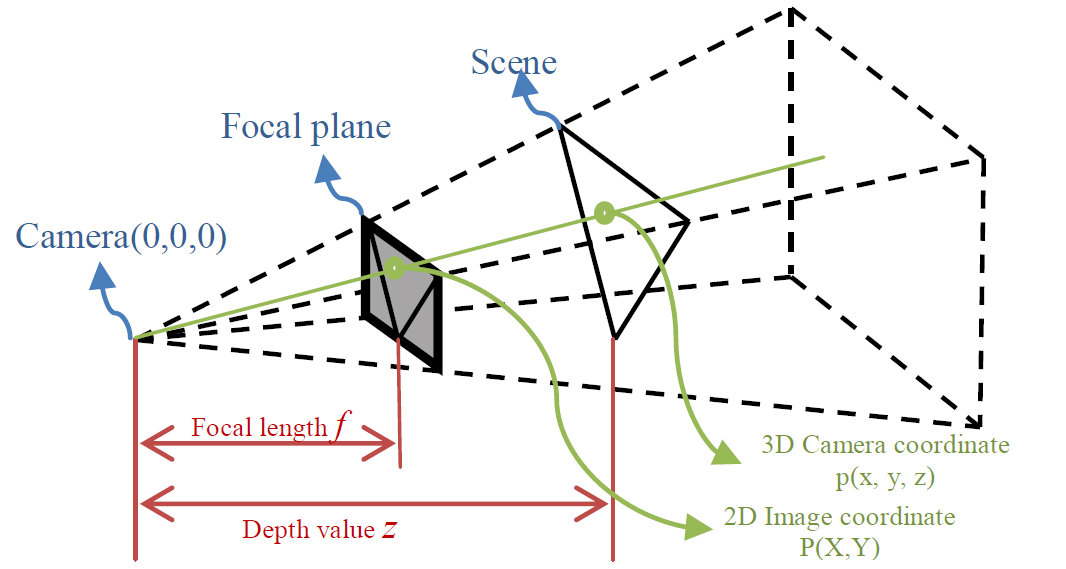
\includegraphics[width=0.8\linewidth]{./figure/perspective.pdf}
\caption{Perspective projection model which is used in this paper for retrieve the 3D point cloud from Kinect.}
\label{f:perspective}
\end{figure}
A perspective projection model (see Figure \ref{f:perspective}) is used to tackle this issue. We set the camera position on the origin of the world coordinate system and set the positive z-axis as the camera's viewing direction. The focal plane is located at a distance $f$ in front of the camera. A 3D point $p_{3D}(x,y,z)$ one the surface of an object in the scene is projected to a 2D pixel $P_{2D}(X,Y)$ on the 2D focal plane. We can derive the geometrical relation between the 3D vertex and the 2D pixel from the rule of similar triangle, see Figure \ref{f:similartri}.
\begin{figure}
\centering
\includegraphics[width=1.0\linewidth]{./figure/similartriangle.pdf}
\caption{Illustration of rule of similar triangle which specifies the relation between $p_{3D}(x,y,z)$ and $P_{2D}(X,Y)$}
\label{f:similartri}
\end{figure}
We can acquire the technical specification \emph{focal length $f$} from performing camera calibration or simply from asking the camera's producer. The transformation of depth map to point cloud can be inferred as the following:
\begin{equation}
p_{i} = (x_{i},y_{i},z_{i}) = (z_{i}\times\dfrac{X_{i}}{f}, z_{i}\times\dfrac{Y_{i}}{f}, z_{i})
\end{equation}

% ------------------------ %
%                          %
%       Nose Detection     %
%                          %
% ------------------------ %
\section{Nose Detection}
\label{s:nose detection}
\begin{figure}
\centering
\includegraphics[width=1.0\linewidth]{./figure/noseDetection.pdf}
\caption{Flow chart of the nose detection procedure: (1) Set a searching window (ROI). (2) Generation the corresponding point cloud for the ROI. (3) Inversely rotate the point cloud. (4) Search the point with smallest z-value.}
\label{f:noseDetect}
\end{figure}

\begin{figure}
\centering
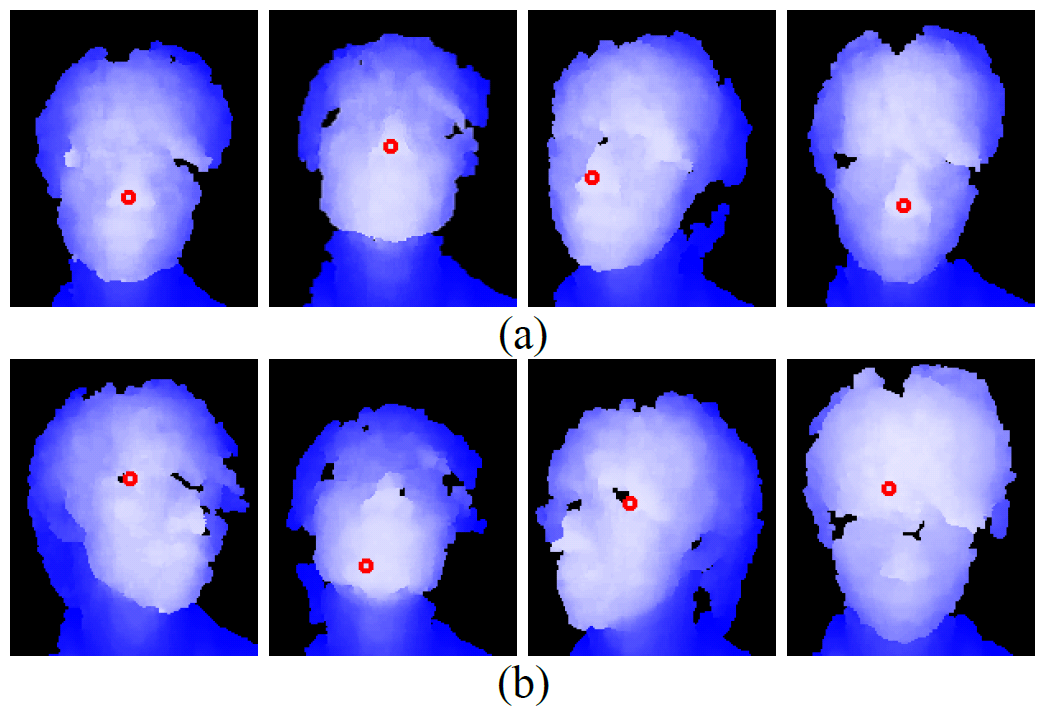
\includegraphics[width=0.7\linewidth]{./figure/nd_nearest.png}
\caption{The corresponding pixel of nose tip has the smallest depth value among the entire depth map when the head rotation is restricted to a narrow range of angles (a), while other parts of the human head will take over the shallowest position (b) when the rotation exceeds the limitation range. Red circle illustrates the detected shallowest point.}
\label{f:nd_nearest}       % Give a unique label
\end{figure}

As mentioned in \ref{s:architecture}, both of the proposed head motion tracking approaches require a nose detection procedure prior to the pose estimation procedure. Figure \ref{f:noseDetect} shows the detailed work flow of this nose detection procedure. 

To detect the user's nose from the depth map, we made an assumption that the nose tip is always the nearest part to the camera among the entire head. Therefore, the corresponding pixel of the nose tip on the depth map holds the smallest depth value. In other words, the pixel which has the smallest depth value within the captured depth map is considered to be the nose tip pixel. In our experiments, this assumption works without any problems as long as the freedom of head rotation is restricted to a narrow range of angles, see Figure \ref{f:nd_nearest}(a).

However, it is obvious that when the user turn his head with larger angles, other parts of human head become closer to the camera than the nose is, then the assumption fails. For example, glasses or cheek will holds the smallest depth value when the yaw angle goes beyond about $\pm{20^{\circ}}$ while chin or fringe will hold the smallest depth value when the pitch angle goes beyond about $\pm{15^{\circ}}$, see Figure \ref{f:nd_nearest}(b). 

A method is proposed in this thesis to handle this issue, named \emph{``inverse rotation''}. The main idea is: When doing motion tracking, we always have temporal informations at hand which are the results estimated from previous frames, and we should make use of these informations. Since a human can only turn his head with small angles within a short moment such as one thirtieth of a second, the relative difference of rotating angles between two consecutive frames will always satisfy our assumption mentioned above. As a result, we apply an inverse rotation matrix to the point cloud captured at time $t$ with the motion parameters estimated at time $t-1$, see Equation \ref{e:ivsRot}:
\begin{equation}
\begin{aligned}
p^{inv}_{i,t} &= R^{-1}_{t-1}p_{i,t}\\
&= [R(\theta _{t-1})R(\psi _{t-1})R(\phi _{t-1})]^{-1}p_{i,t}\\
&= R(\phi _{t-1})^{-1}R(\psi _{t-1})^{-1}R(\theta _{t-1})^{-1}p_{i,t}\\
&= R(-\phi _{t-1})R(-\psi _{t-1})R(-\theta _{t-1})p_{i,t}
\end{aligned}
\label{e:ivsRot}
\end{equation}
In Equation \ref{e:ivsRot}, $p_{i,t}$ indicates the $i$-th point of the point cloud captured at time $t$, while $p^{inv}_{i,t}$ indicates the corresponding position of $p_{i,t}$ after inverse rotation transformation. The $\theta _{t-1}$, $\psi _{t-1}$, and $\phi _{t-1}$ are the estimated results of pitch, yaw, and roll angles at time $t-1$. $R$ refers to the same rotation matrix as Equation \ref{e:rbt}. After the inverse rotation transformation, the point cloud represents a head faces straight forward to the camera with only a tiny range of variation. Therefore, the corresponding point of the nose tip still holds the smallest z-value. As a consequence, by applying the proposed nose detection method, we can always successfully locate and track the position of the user's nose tip as long as it's been captured in the current depth map. 

\begin{figure}
\centering
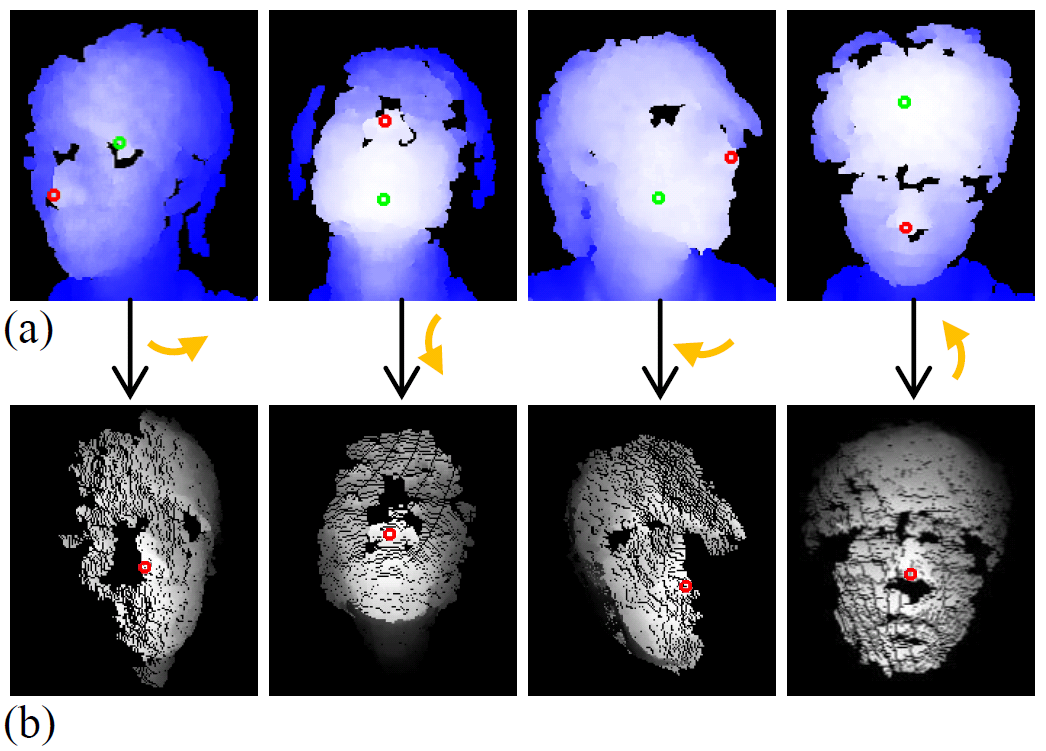
\includegraphics[width=0.7\linewidth]{./figure/inverserotation.png}
\caption{An inverse rotation transform is applied to the whole point cloud (a) to rotate the head back to the normal pose (b). Green circle indicates the shallowest point while red circle indicates the new shallowest point after inverse rotation.}
\label{f:invRot}
\end{figure}

Figure \ref{f:invRot}(a) illustrates a scenario that the user rotates his head with angles so large that other parts of his head become the nearest part to the camera instead of the nose tip. The green circles in Figure \ref{f:invRot}(a) mark up the smallest depth value pixels without doing inverse rotation transformation first. It is clear that locating the nose tip by purely finding the pixel with the smallest depth value in such conditions will definitely fail. Figure \ref{f:invRot}(b) shows point clouds that are inversely rotated from point clouds in \ref{f:invRot}(a). Red circles in Figure \ref{f:invRot}(b) show the points with smallest depth values among the inverse rotated point clouds, and their corresponding pixels in the depth map are marked by the red circles in Figure \ref{f:invRot}(a).

\begin{figure}
\centering
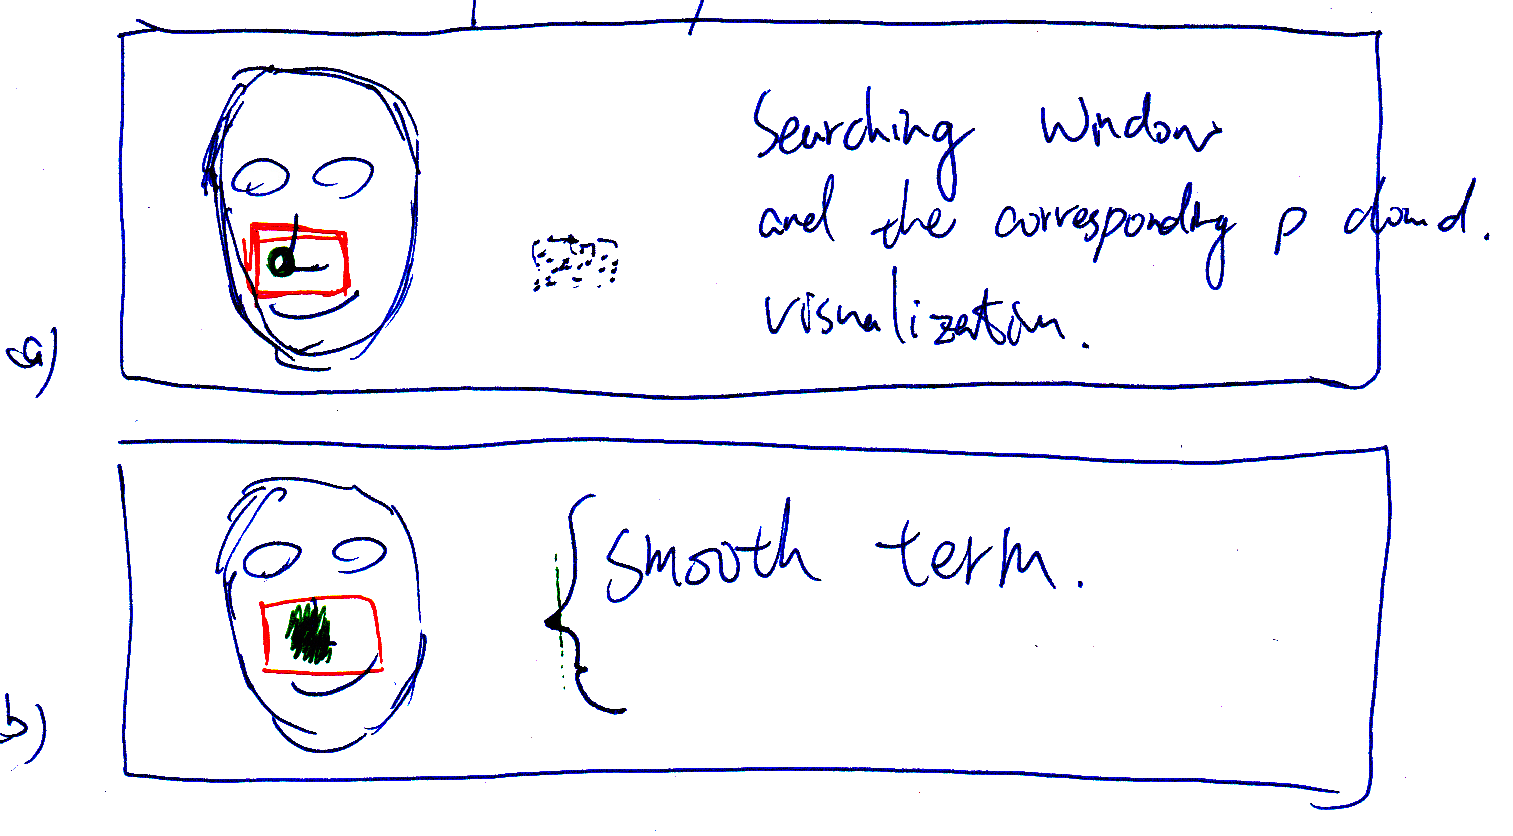
\includegraphics[width=1.0\linewidth]{./figure/noseROI_Smooth.pdf}
\caption{Figure (a) shows the temporal view of the nose tracking results in a period of 10 seconds without doing smoothing process. Figure (b) shows the results with smoothing process. }
\label{f:noseROI Smooth}
\end{figure}
\begin{figure}
\centering
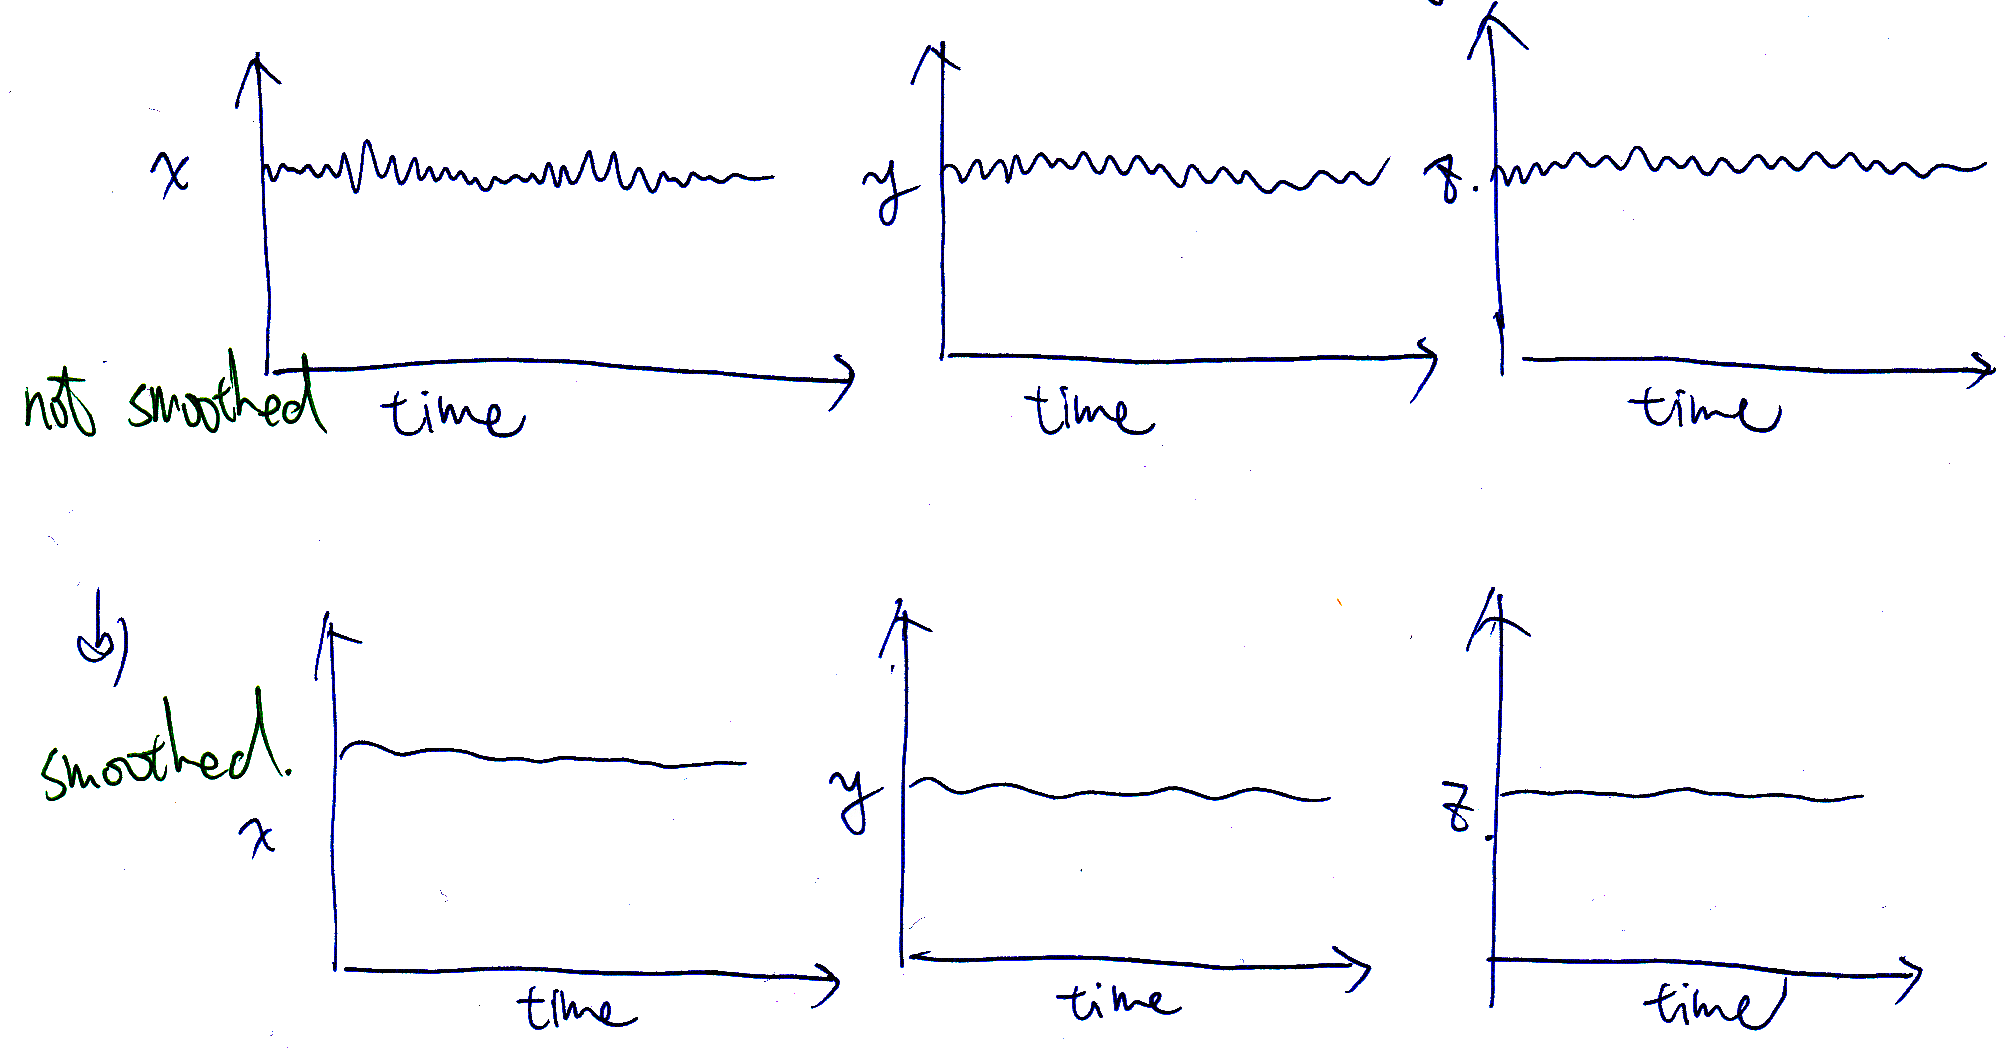
\includegraphics[width=1.0\linewidth]{./figure/noseSmoothCompare.pdf}
\caption{Figure (a) shows the searching window and the corresponding point cloud of the pixels inside the window. Figure (b) shows the smoothness term. }
\label{f:nose Smooth Compare}
\end{figure}
In practical implementation, we need to further increase the robustness and decrease the computational cost for this nose detection procedure. A searching window can achieve both requirements. Reminding that human head can not perform large motions within a short moment, which refers to the time period between two consecutive frames, we reduce the nose searching area to a small window instead of the entire depth map. Note that the center of a searching window at time $t$ is set at the nose position previously estimated at time $t-1$, while there is no searching window set at the very beginning of the system. Recalling that there's a serious flickering issue with the depth camera mentioned in Section \ref{s:hardware}, it affects the result of nose detection, too. The noise and inaccuracy of the acquired depth map cause the nose detection to have a jittering problem. To tackle this jittering issue, we propose to calculate the center position of the subset ${(x_{i},y_{i},z_{i})|z_{i}\leq z_{nose}+5}$ of the inversely rotated point cloud . Figure \ref{f:noseROI Smooth}(b) shows the smoothness term, red pixels on the left figure indicate the subset ${(x_{i},y_{i},z_{i})|z_{i}\leq z_{nose}+5}$ while the right figure is the side view. Figure \ref{f:nose Smooth Compare}(a) shows the temporal view of the nose tracking results in a period of 10 seconds without doing smoothing process. The consecutively detected nose positions form a motion with high frequency. Figure \ref{f:nose Smooth Compare}(b) shows the results with smoothing process.

% ------------------------ %
%                          %
%   Least Square Solution  %
%                          %
% ------------------------ %
\section{Head Pose Estimation: Least Square Solution}
\label{s:method1}
\begin{figure}
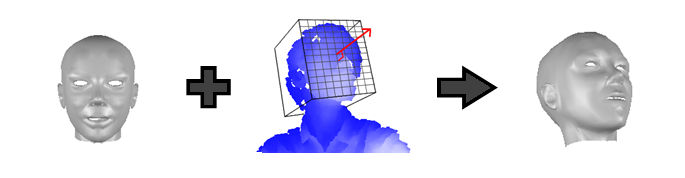
\includegraphics[width=1.0\linewidth]{./figure/M1_highlevel.png}
\caption{The high level idea of least square solution to the head pose estimation. Assuming that a head can be approximated by a bounding box, then the motion of this box can stands for the motion of the head.}
\label{f:m1_high}       % Give a unique label
\end{figure}
In this section, we are going to talk about one of the proposed 3D head motion tracking approach. Assuming that a head can be approximated by a bounding box, then the motion of this box can stands for the motion of the head (see Figure \ref{f:m1_high}). We propose to reconstruct the 6 degrees of freedom for this bounding box. 

\paragraph{Translation Estimation}
The estimation on the three directional translation parameters is the easier part of the motion tracking task. By calculating the center position of the point cloud, translation parameters can be easily estimated:
\begin{equation}
(t_{x},t_{y},t_{z})=\frac{\sum_{i=1}^n{(x_{i},y_{i},z_{i})}}{N}
\end{equation}

\paragraph{Rotation Estimation}
\begin{figure}
\centering
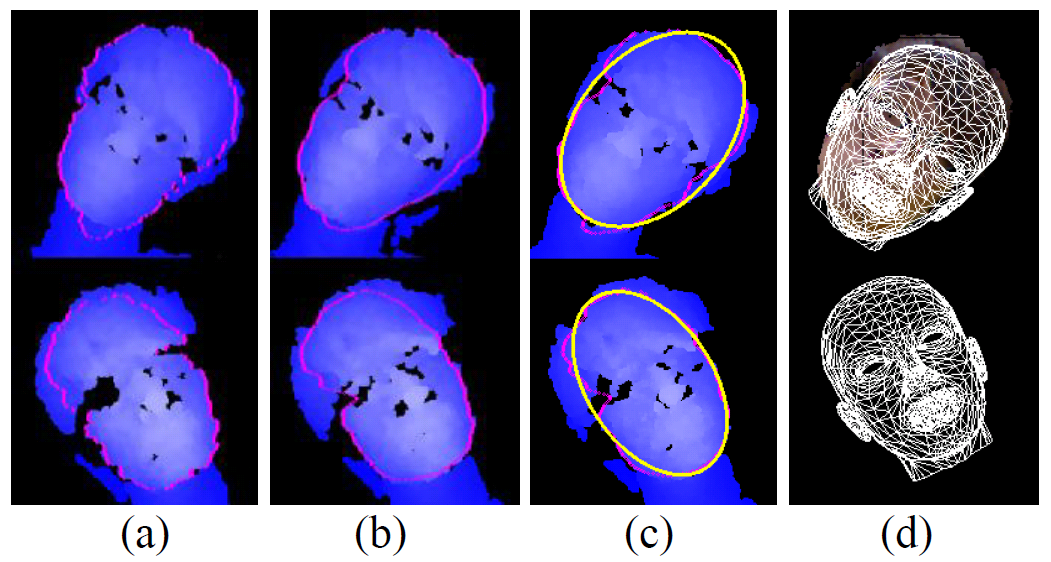
\includegraphics[width=0.7\linewidth]{./figure/ellipsefitting.png}
\caption{Detect the boundary of user’s head (a), and smooth the boundary by averaging neighboring points (b). Fit an ellipse that best matches the smoothed head boundary(c), and apply the angle of the result ellipse to the virtual avatar.}
\label{f:ellipse}       % Give a unique label
\end{figure}

We propose a novel approach for rotation estimation. The estimation can be divided into two parts. First, we reconstruct the frontal plane of the bounding box. The normal vector of this plane solves two degrees of freedom of the head pose information, which are pitch angle and yaw angle. On the other hand, the roll angle can be estimated by reconstruct an ellipse that fits the head's contour. 

In roll angle estimation process, in order to find a bested fitted ellipse to the head, we locate the contour of the head first. A depth threshold value is used to filter out the background pixels, then the leftmost and the rightmost pixels in each row represent the contour (See Figure \ref{f:ellipse}(a)). However, since the captured depth information through Kinect is quite noisy, the detected contour fluctuates and causes the estimated roll angle to have a jittering problem. For example, if we drive a virtual avatar with the estimated roll angle, the virtual avatar will tremble even there is no head motions. Therefore, we add a smoothing process to handle this issue. We apply an ``averaging filter'' (, which is equal to a low-pass filter) to the pixel set of head contour. The smoothed head contour is shown in Figure \ref{f:ellipse}(b).

After the smoothing process, we find an ellipse that is best fitted to the contour pixels by least square error method. Figure \ref{f:ellipse}(c) shows the best fitted ellipse. Then we take the rotation angle of the best fitted ellipse as the estimated roll angle. Figure \ref{f:ellipse}(d) shows the result.

\paragraph{Pitch and Yaw Angles Estimation}
\begin{figure}
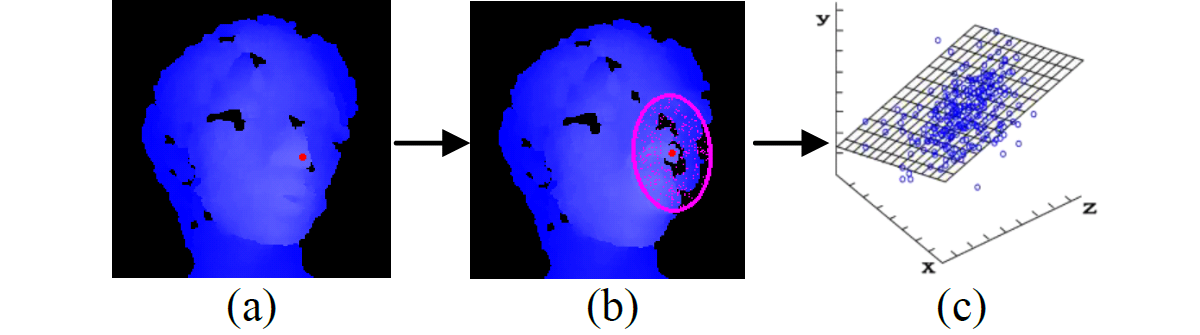
\includegraphics[width=1.0\linewidth]{./figure/lsqp.png}
\caption{Detect and track user’s nose (a) and sample several points from the nose’s neighboring area (b) and apply least square error approach to get the best fitted plane to the sample points (c).}
\label{f:lsqp}       % Give a unique label
\end{figure}
Human faces can be roughly considered as a plane. The normal vector of this plane can represent the orientation of the actor’s head. Our goal is to reconstruct this plane. Figure \ref{f:lsqp} illustrates the work flow of the plane fitting process. The first step is nose detection, because the nose is always the center part of the human face thus we can do sampling on the frontal face as long as we know the exact location of the nose. After the location of the nose tip is found by the approach described in Section \ref{s:nose detection}, the second step is sampling. We randomly sample $300$ pixels around the nose from the depth map, (Figure \ref{f:lsqp sampling}). We show that the sample number $300$ is sufficient in our experiments. However, owing to the least square solution $A^{T}Ax=A^{T}b$, increasing the sample number will not cause computational problems. For the third step, we generate a point cloud for the sample pixels by the approach described in Section \ref{s:point cloud gen}, and find the best fitted plane of the sample point cloud in 3D space.
\begin{figure}
\centering
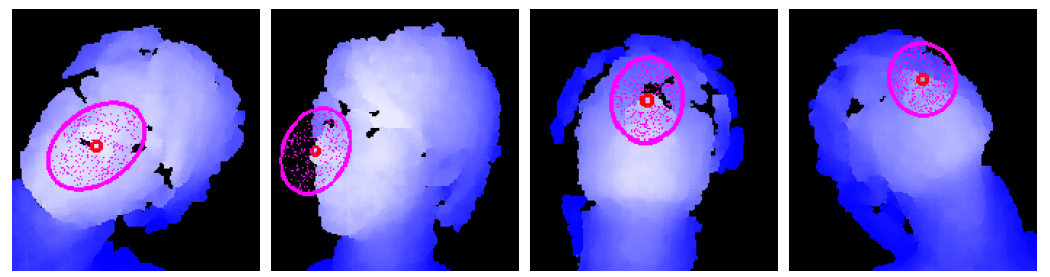
\includegraphics[width=0.7\linewidth]{./figure/lsqpSampling.png}
\caption{We sample 300 pixels from the defined face area. If any sample pixels have no depth value, we just ignore them.}
\label{f:lsqp sampling}       % Give a unique label
\end{figure}
Assume the algebraic expression of the best fitted plane is $Ax+By+C=z$, the coefficients $(A,B,C)$ can be obtained by solving the following equation:
\begin{equation}
\begin{bmatrix}
\sum_{i=1}^{n}{x_{i}^2} 	& \sum_{i=1}^{n}{x_{i}y_{i}}	& \sum_{i=1}^{n}{x_{i}}	\\
\sum_{i=1}^{n}{x_{i}y_{i}} 	& \sum_{i=1}^{n}{y_{i}^2}		& \sum_{i=1}^{n}{y_{i}}	\\
\sum_{i=1}^{n}{x_{i}} 		& \sum_{i=1}^{n}{y_{i}}			& \sum_{i=1}^{n}{1}	
\end{bmatrix}
\begin{bmatrix}
A	\\
B	\\
C
\end{bmatrix}
=
\begin{bmatrix}
\sum_{i=1}^{n}{x_{i}z_{i}}	\\
\sum_{i=1}^{n}{y_{i}z_{i}}	\\
\sum_{i=1}^{n}{z_{i}}
\end{bmatrix}
\end{equation}

\begin{figure}
\centering
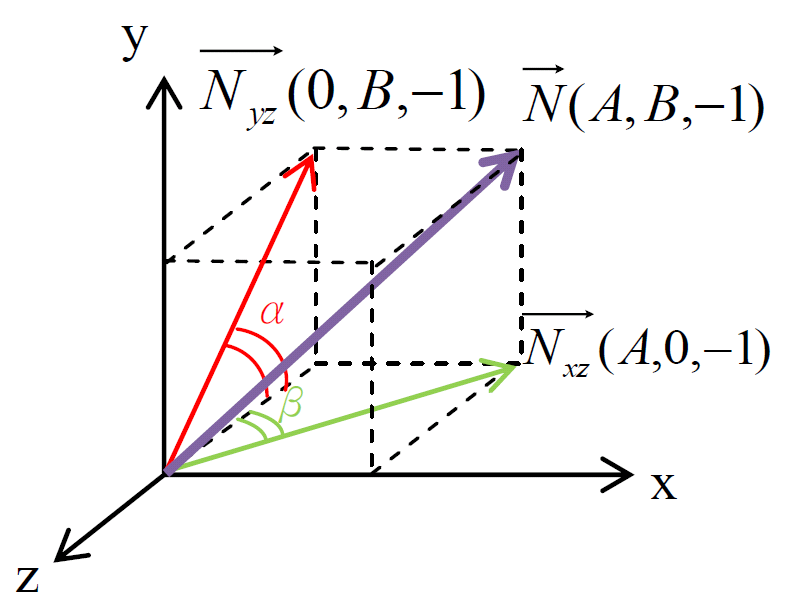
\includegraphics[width=0.5\linewidth]{./figure/vec2angle.png}
\caption{The relation between normal vector $\vec{N}$ and pose parameter {yaw,pitch}. $\alpha$ denotes pitch angle while $\beta$ denotes yaw angle.}
\label{f:vec2angle}       % Give a unique label
\end{figure}

We then transform the normal vector $\vec{N}(A,B,-1)$ to yaw and pitch angles. Figure \ref{f:vec2angle} illustrates the relation between normal vector $\vec{N}(A,B,-1)$ and pose parameter {yaw,pitch}. $\alpha$ is the angle between $\vec{N}_{yz}$ and negative z-axis and denotes pitch angle, where $\vec{N}_{yz}(0,B,-1)$ is obtained by projecting $\vec{N}(A,B,-1)$ onto y-z plane. On the other hand, $\beta$ is the angle between $\vec{N}_{xz}$ and negative z-axis and denotes yaw angle, where $\vec{N}_{xz}(A,0,-1)$ is obtained by projecting $\vec{N}(A,B,-1)$ onto x-z plane. Finally, the pitch angle $\alpha$ is obtained by calculating $\tan^{-1}{(B)}$ while the yaw angle $\beta$ is obtained by calculating $\tan^{-1}{(A)}$.

Thanks to the fact that both of the plane and ellipse fitting process have least square solution, the proposed approach has low computational cost and gives fully real-time responses (30fps) without needing the GPU speedup.

% ------------------------ %
%                          %
%   Least Square Solution  %
%                          %
% ------------------------ %
\section{Head Pose Estimation: Optimization Solution}
\label{s:Method2}


In this section, we will discuss the second proposed method in detail. The motivation to develop this method is simply a desire to solve the limitation of the previous method - lack of precision. In order to obtain preciser motion vectors, we regard the problem as an optimization problem. However, most of the optimization methods have high computational cost. We will also specify how we reduce the computational cost and thus make the system remain 30 fps without GPU acceleration.

This method has an initialization step that requires the user to take a snapshot of depth map for his frontal face. The 3D point cloud retrieved form this depth map will be mentioned as ``model point cloud'' and denoted as $P_{M}$ later in this chapter. Figure \ref{f:modelPC} shows a $P_{M}$ in different viewing angle. The system then build a kd-tree for this model which will be used for nearest point searching. Note that it takes only about 50 milliseconds to build the kd-tree so that the user will not wait for this process. In the head motion tracking part, same as method 1, we detect the nose by the proposed inverse rotation method and sample several points around it. These sample points will be mentioned as ``sample point cloud'' and denoted as $P_{S}$ later in this chapter. Different from method 1, the number of samples directly affect the computation time of this method. The higher the number is, the more precise the results will be, and the longer response time will the system need. Our experiments show that 30 is enough for this number to make the results precise enough to be compared with state-of-the-art approaches and still gives real-time responses in the same time. Figure \ref{f:samplePC} shows an example of a sample point cloud in different viewing angle, noted that we sampled 70 points in this example to have a more clear visualization. 


\begin{figure}
\centering
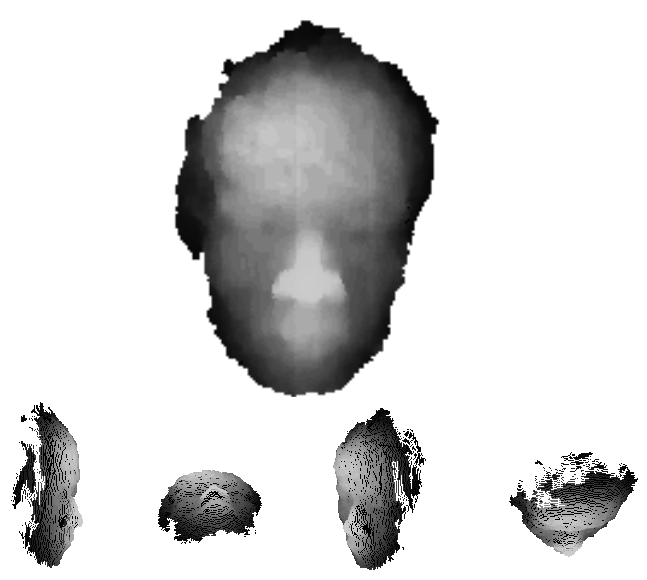
\includegraphics[width=0.7\linewidth]{./figure/modelPointCloud.png}
\caption{An example of a model point cloud created from a single snapshot that the user is required to face the depth camera either at the beginning of the on-line process or in an additional off-line process. }
\label{f:modelPC}
\end{figure}

\begin{figure}
\centering
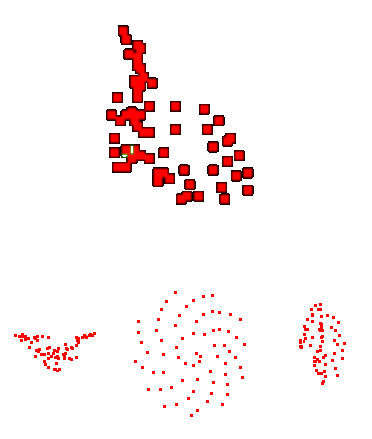
\includegraphics[width=0.5\linewidth]{./figure/samplePointCloud.png}
\caption{An example of a sample point cloud which is sparsely sampled from the input depth map.}
\label{f:samplePC}
\end{figure}

After obtaining the sample point cloud and the model point cloud, we define a metric to measure the distance between them. A rigid body transformation module is described here:
\begin{equation}
p'_{i} =
\begin{bmatrix}x'_{i}\\y'_{i}\\z'_{i}\end{bmatrix}
= R(\theta,\psi,\phi)
\begin{bmatrix}x_{i}\\y_{i}\\z_{i}\end{bmatrix}
+ 
\begin{bmatrix}t_{x}\\t_{y}\\t_{z}\end{bmatrix}
= Rp_{i} + T
\label{rbt}
\end{equation}
where R is a 3$\times$3 rotation matrix represented in terms of roll, yaw and pitch angles, T is a translation vector, and $p_{i}$ indicates the point of the sample point cloud $P_{S}$. For simplicity, we rewrite Equation \ref{rbt} as:
\begin{equation}
p' = RBT(p)
\label{rbtSimple}
\end{equation}
Knowing that a set of input parameters of this rigid body transformation is identical to the 6-DoF head motion vector, our goal is to obtain the best motion vector which is able to match $P_{S}$ to $P_{M}$ by rigid body transformation. The energy function is defined as following:
\begin{equation}
E(\theta,\psi,\phi,t_{x},t_{y},t_{z},P_{S},P_{M})=\sum_{p}^{p\in P_{S}}min(d(RBT(p),P_{M}))
\end{equation}
where $min(d(RBT(p),P_{M})$ indicates the minimum distance from $p'$(,also denoted as RBT(p)) to the model point cloud. This minimum distance can be inferred by calculating the L2 distance between $p'$ and its corresponding nearest point in $P_{M}$ searching from the kd-tree built at the beginning. For simplicity, we replace the notation of the objective function with $E_{a}$ where $a=(\theta,\psi,\phi,t_{x},t_{y},t_{z})$ and $(P_{S},P_{M})$ are omitted since they are fixed. Our task is then specified as:
\begin{equation}
Result = a^{*} = \emph{arg\: min} (E_{a})
\end{equation}
To solve this equation, the concept of gradient decent algorithm is applied:
\begin{equation}
\label{gda}
x^{k+1}=x^{k}-\alpha_{k}\triangledown f(x^{k})
\end{equation}
The coefficient $\alpha_{k}$ is a positive scalar called step size. The algorithm finds the minimum value of $f(x)$ by iteratively updating $x$ such that $f(x^{k+1})$<$f(x^{k})$, where k is the number of iterations. For our task, Eq.~\ref{gda} can be rewritten as:
\begin{equation}
\label{gdaE}
a^{k+1}=a^{k}-\alpha_{a}\triangledown E(a^{k})
\end{equation}
Since our objective function is non-differentiable, we can't calculate the gradient $\triangledown E$, so we approximate the gradient by evaluating on twelve possible directions:

\begin{equation}
\begin{aligned}
\triangledown_{1}&=\begin{bmatrix}1\\0\\0\\0\\0\\0\end{bmatrix}
\triangledown_{2}&=\begin{bmatrix}-1\\0\\0\\0\\0\\0\end{bmatrix}
\triangledown_{3}&=\begin{bmatrix}0\\1\\0\\0\\0\\0\end{bmatrix}
\triangledown_{4}&=\begin{bmatrix}0\\-1\\0\\0\\0\\0\end{bmatrix}
\triangledown_{5}&=\begin{bmatrix}0\\0\\1\\0\\0\\0\end{bmatrix}
\triangledown_{6}&=\begin{bmatrix}0\\0\\-1\\0\\0\\0\end{bmatrix} \\
\triangledown_{7}&=\begin{bmatrix}0\\0\\0\\1\\0\\0\end{bmatrix}
\triangledown_{8}&=\begin{bmatrix}0\\0\\0\\-1\\0\\0\end{bmatrix}
\triangledown_{9}&=\begin{bmatrix}0\\0\\0\\0\\1\\0\end{bmatrix}
\triangledown_{10}&=\begin{bmatrix}0\\0\\0\\0\\-1\\0\end{bmatrix}
\triangledown_{11}&=\begin{bmatrix}0\\0\\0\\0\\0\\1\end{bmatrix}
\triangledown_{12}&=\begin{bmatrix}0\\1\\0\\0\\0\\-1\end{bmatrix}
\end{aligned}
\end{equation}


At $(k+1)th$ iteration, all these twelve directions are evaluated by setting $a^{k+1}=a^{k}-\alpha_{a}\triangledown_{i}$. We choose the one with smallest $E(a^{k+1})$ to be the best parameter set $\hat{a}^{k+1}$. The iteration stops either the maximum number N of iterations achieved or the value of $E(\hat a^{k+1})$ is smaller than a defined error threshold. As a result, the optimized parameter set for matching the sample point cloud to the model point cloud is obtained ($\hat a$). Then the opposite parameter set can be used for matching the model point cloud to the sample point cloud. In brief, the 6-Dof head motion vector is obtained and our goal is achieved. Figure \ref{f:icp nose} shows an example of the iterative procedure. The iteration starts from the column on the left and converges at the column on the right.

\begin{figure}
\centering
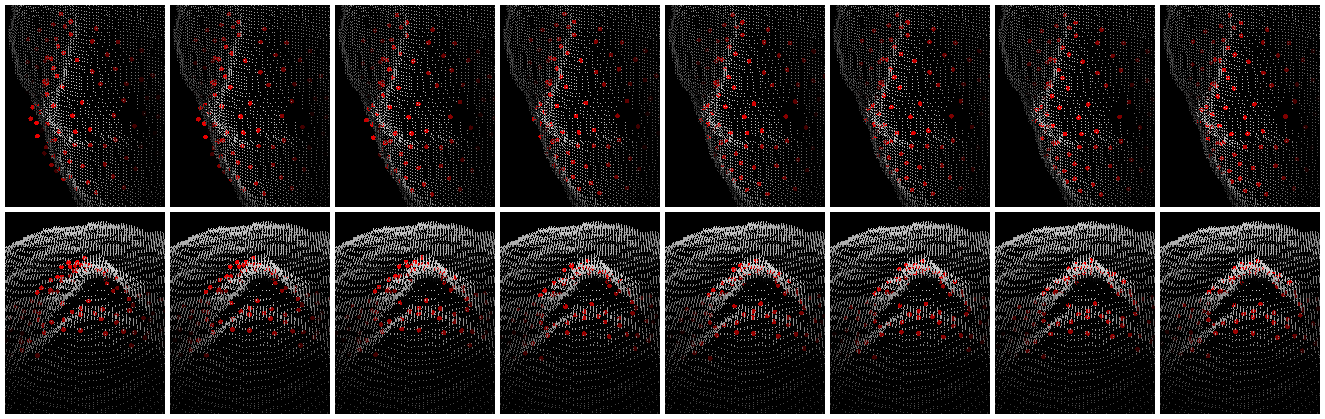
\includegraphics[width=1.0\linewidth]{./figure/ICP_Nose_Hilight1.png}
\caption{The process of the iterative optimization method. The iteration starts from the column on the left and converges at the column on the right.}
\label{f:icp nose}
\end{figure}

% ------------------------ %
%                          %
%   Least Square Solution  %
%                          %
% ------------------------ %
\section{Smooth Filter}
\label{s:smooth filter}
Owing to the high noise of the acquired depth maps, there is an inconsistent issue with the tracked motion vectors. In other words, when we make an animation by retargeting the estimated motion vector stream to a virtual character, we can easily observe the virtual character trembling. A common solution is to adopt a low pass filter. Using the average motion vector of the latest several outputs can alleviate the severity of trembling. Nevertheless, a time lag shows up as well. 
\begin{figure}
\centering
\includegraphics[width=0.6\linewidth]{./figure/DynamicFilter.pdf}
\caption{The dynamic weighted averaging filter referenced from \cite{Weise:11:RPBFA}.}
\label{f:dynamic filter}
\end{figure}
We apply a dynamic weighted averaging filter similar to that of \cite{Weise:11:RPBFA} to solve this problem. We independently filter the translation and rotation vectors. For a translation or rotation vector $t_{i}$ at the current time frame i, we compute the smoothed vector as weighted average in a window of size k as
\begin{equation}
t_{i}^{*}=\dfrac{\sum_{j=0}^{k}w_{j}t_{i-j}}{\sum_{j=0}^{k}w_{j}}
\end{equation}
where $t_{i-j}$ denotes the vector at frame $i-j$. The weights $w_{j}$ are defined as
\begin{equation}
w_{j}=e^{-j\dot H\dot max_{l\in [1,k]}\parallel t_{i}-t_{i-l} \parallel},
\end{equation}
with a constant H that we empirically determine independently for rotation and translation based on the noise level of a static pose. We use a window size of $k=5$ for all our experiments.